\chapter{Measures and function spaces} \label{chap:Leb-spaces}
\section{\texorpdfstring{$L^p$}{Lp} when \texorpdfstring{$1 \leq p < \infty$}{1 <= p < infinity}} \label{sec:Lp-1-infty}
Let $(X,\A,\mu)$ be the underlying measure space and $0< p < \infty$. We define the \df[p norm@$p$ norm]{$p$-norm} of a measurable function $f$ by \[
    \nm{f}_{p} = \biggl(\int_X \abs{f}\,d\mu\biggr)^{1/p} \in [0,\infty].
\] The \df[Lp space-cal@$\mathcal{L}^p$ space]{$\mathcal{L}^p$ space} is the space of measurable functions with finite $p$-norms.

The space $\mathcal{L}^p$ is not quite a normed space under $\nm{\blank}_p$. We will soon see that only when $1 \leq p < \infty$, $\nm{\blank}_p$ will become a seminorm on $\mathcal{L}^p$. Hence if we consider the equivalence classes of functions in $\mathcal{L}^p$ that are a.e.\ the same, then $\nm{\blank}_p$ becomes a norm. The set of equivalence classes we described here is called the \df[Lp space@$L^p$ space]{$L^p$ space}. We make the appearance of equivalence classes in the definition of $L^p$ spaces implicit in our exposition, as long as it does not need to confusion; for example, we always write a function $f \in L^p$ instead of $f \in \mathcal{L}^p$.

The $L^1$ space of integrable functions have been the sole focus in the previous chapters. In this chapter we will look at the functional analytic structure of the $L^p$ spaces, and touch on their connections to the theory of Fourier analysis.

\begin{namedthm}[Hölder's inequality] \label{thm:Holder-ineq}
    Let $\frac{1}{p} + \frac{1}{q} = 1$, then \[
        \nm{fg}_1 \leq \nm{f}_p\nm{f}_q.
    \]

    ($p$ and $q$ satisfying $\frac{1}{p} + \frac{1}{q} = 1$ are called conjugate exponents.)
\end{namedthm}

\begin{namedthm}[Minkowski's inequality] \label{thm:Minkowski-ineq}
    For $1 \leq p < \infty$, we have $\nm{f+g}_p \leq \nm{f}_p + \nm{g}_p$.
\end{namedthm}

\begin{thm}
    $L^p$ is complete.
\end{thm}

\begin{prop}
    The equivalence class simple functions are dense in $L^p$ hence $L^q \cap L^p$ is dense in $L^p$ (6.7)
\end{prop}

\begin{prop}
    For any finite measure $\mu$ on a metric space, we have $C_b(X)$ is dense in $L^p(\mu)$. \cite[Proposition~3.16]{Ambrosio_2011}
\end{prop}

A separable metric space with Borel $\sigma$-algebra is countably generated. To see this, one can take open balls centered at a countable dense subset with rational radius.

\begin{thm}[{\cite[Proposition~4.3.5]{Cohn_2013}}]
    If $\A$ is countably generated and $\mu$ is $\sigma$-finite, then $L^p(X)$ is separable for $1 \leq p < \infty$. 
\end{thm}

\section{\texorpdfstring{$L^p$}{Lp} when \texorpdfstring{$p = \infty$}{p = infty}}
\begin{thm}
    $L^\infty$ is complete.
\end{thm}

For any Borel measure that assigns positive values to all open sets (e.g., the Lebesgue measure on $\R^d$), we have $\nm{f}_{\infty} = \nm{f}_u$ when $f$ is continuous, since $\{x:\abs{f(x)} > t\}$ is open. Notice that the equivalence class of $(C_b(X),\nm{\blank}_u)$ may be regarded as a closed subspace of $(L^\infty(X),\nm{\blank}_\infty)$, since $(C_b(X),\nm{\blank}_u)$ is complete. It is clear that we do not have the density of $C_b$ in $L^\infty$ in general.

\begin{prop}[{\cite[Proposition~6.10]{folland1999}}]
    For $1 \leq p < q < r \leq \infty $, then $L^p \cap L^r \subseteq L^q$, and \[
        \nm{f}_q \leq \nm{f}_p^\lambda \nm{f}_r^{1-\lambda},
    \] where \[
        \lambda = \frac{q^{-1} - r^{-1}}{p^{-1} - r^{-1}} \in (0,1).
    \]
\end{prop}

\begin{prop}[{\cite[Exercise~6.7]{folland1999}}]
    If $f \in L^p \cap L^\infty$ for some $p < \infty$, then \[
        \nm{f}_\infty = \lim_{q \to \infty} \nm{f}_q.
    \]
\end{prop}

The condition $f \in L^p \cap L^\infty$ enforces $f \in L^q$ for all $q > p$. One might ask if $f \in L^q$ for all $q \geq p$, then $f \in L^\infty$ automatically. This is unfortunately wrong: on the unit interval endowed with the Lebesgue measure, the function $\log(x)$ has finite $L^p$ norm $\Gamma(p+1)^{1/p}$ for all $p < \infty$ (verify this!), and is close to $p/e$ for large $p$. However, the logarithm function is not bounded a.e.

Assume $1\leq p < q \leq \infty$.

\begin{prop}[{\cite[Proposition~6.12]{folland1999}}]
    In a finite measure space, $L^p \supseteq L^q$, with \[\nm{f}_p \leq \nm{f}_q \mu(X)^{\frac{1}{p} - \frac{1}{q}}.\] The case $\mu(X) = 1$ is nice.
\end{prop}

\begin{prop}[{\cite[Proposition~6.11]{folland1999}}]
    Let $A$ be any set, then $\ell^p(A) \subseteq \ell^q(A)$, with $\nm{f}_p \geq \nm{f}_q$.
\end{prop}

Think about in $\R^2$, the $\ell^1$-ball is contained in the $\ell^2$-ball,..., and is all contained in the $\ell^\infty$-ball. But when thinking about abstract $L^p$ spaces, the direction of containment is reversed. The geometry is different.

\section{Hilbert spaces and \texorpdfstring{$L^2$}{L2}}

There is a canonical choice of orthonormal basis on the Hilbert space $L^2[0,1]$.

Haar function



\begin{figure}
    \centering
    \subfloat[$\phi_{0,0}$]{
            \begin{tikzpicture}
            \begin{axis}[
  axis x line=middle, axis y line=left,
  ymin=-1.6, ymax=1.6, ytick={-1,0,1}, ylabel=$y$,
  xmin=0, xmax=1.3, xtick={0,1}, xlabel=$x$,
  domain=0:1, % added
    height=1.8in, width=1.8in
]
                \addplot[blue,thick,samples at={0,1}] {1};
            \end{axis}
        \end{tikzpicture}
    }
    \hspace{.5in}
    \subfloat[$\phi_{1,0}$]{
            \begin{tikzpicture}
            \begin{axis}[
  axis x line=middle, axis y line=left,
  ymin=-1.6, ymax=1.6, ytick={-1,0,1}, ylabel=$y$,
  xmin=0, xmax=1.3, xtick={0,1}, xlabel=$x$,
  domain=0:1, % added
    height=1.8in, width=1.8in
]
                \addplot[blue,thick,unbounded coords=jump,samples at={0,0.49,0.50,0.51,1}] {and(x >= 0,x < 1/2) * 1 + and(x > 1/2,x <= 1) * (-1) + (x == 1/2) * inf};
            \end{axis}
        \end{tikzpicture}
    } \\

    \subfloat[$\phi_{2,0}$]{
            \begin{tikzpicture}
            \begin{axis}[
  axis x line=middle, axis y line=left,
  ymin=-1.6, ymax=1.6, ytick={-1,0,1}, ylabel=$y$,
  xmin=0, xmax=1.3, xtick={0,1}, xlabel=$x$,
  domain=0:1, % added
    height=1.8in, width=1.8in
]
                \addplot[blue,thick,unbounded coords=jump,samples at={0,0.24,0.25,0.26,0.49,0.50,0.51,0.74,0.75,0.76,1}] {and(x >= 0,x < 1/4) * 1 + and(x > 1/4,x < 1/2) * (-1) + (x == 1/4) * inf + (x == 1/2) * inf + (x > 1/2) * (0)};
            \end{axis}
        \end{tikzpicture}
    }
    \hspace{.5in}
    \subfloat[$\phi_{2,1}$]{
            \begin{tikzpicture}
            \begin{axis}[
  axis x line=middle, axis y line=left,
  ymin=-1.6, ymax=1.6, ytick={-1,0,1}, ylabel=$y$,
  xmin=0, xmax=1.3, xtick={0,1}, xlabel=$x$,
  domain=0:1, % added
    height=1.8in, width=1.8in
]
                \addplot[blue,thick,unbounded coords=jump,samples at={0,0.24,0.25,0.26,0.49,0.50,0.51,0.74,0.75,0.76,1}] {and(x >= 1/2,x < 3/4) * 1 + and(x > 3/4,x <= 1) * (-1) + (x == 3/4) * inf + (x == 1/2) * inf + (x < 1/2) * (0)};
            \end{axis}
        \end{tikzpicture}
    }
         \caption[]{Haar basis functions}
        \label{fig:Haar-basis}
\end{figure}

Every Hilbert space with orthonormal basis $\{e_\alpha\}_{\alpha \in A}$ is unitarily isomorphic to $\ell^2(A)$.

Every infinite-dimensional separable Hilbert space is unitarily isomorphic to $L^2[0,1]$.

\section{Duality of \texorpdfstring{$L^p$}{Lp}}

\begin{namedthm}[Riesz representation theorem ($L^p$ spaces)]
    Let $(X,\A,\mu)$ be a $\sigma$-finite measure space. and let $1\leq p<\infty$. For every $\Phi \in (L^p)^*$, there is a unique $f \in L^q$ such that for all $g \in L^p$, we have \[
        \Phi(g) = \int fg\,d\mu.
    \] Meanwhile $\nm{\Phi} = \nm{f}$, which means $(L^p)^*$ is isometrically isomorphic to $L^q$.

    The statement above remains true if $\mu$ is not $\sigma$-finite, as long as $1 < p < \infty$.
\end{namedthm}

\section{Convolutions and smooth approximation}
Let $f$ and $g$ be measurable, the \df{convolution} of $f$ and $g$ is the function \[
    f * g(x) = \int f(x - y)g(y)\,d\mu(y)
\] for all $x$ such that the integral exists.

\begin{namedthm}[Young's inequality]
    For $1 \leq p,q,r\leq \infty$ and $\frac{1}{p} + \frac{1}{q} = \frac{1}{r} + 1$, then if $f \in L^p$ and $g \in L^q$, then $f * g$ is defined a.e.\ (if $r = \infty$ then everywhere) and is in $L^r$, with \[
        \nm{f * g}_{r} \leq \nm{f}_p\nm{g}_q.
    \]
\end{namedthm}

It is clear that we can 

\section{Riesz' theorems and convergence of measures}\label{sec:Riesz-thm}
We will let $X$ always be a locally compact metric space in this section. All results in this section can be generalized to locally compact Hausdorff spaces with more sophisticated topological tools and arguments.

\subsection{The topology of locally compact spaces}

For a Radon measure $\mu$ on a locally compact metric space $X$, we have $C_c(X)$ is dense in $L^p(\mu)$. (Folland 7.9)

\begin{namedthm}[Urysohn's lemma] (locally compact spaces) \label{thm:Urysohn-local-compact}
    Let $X$ be a locally compact metric space, and let $K$ be compact and $U$ be open in $X$ such that $K \subseteq U$.
    \begin{enumerate}
        \item \label{enu:precompact-in-between} We can construct a precompact open set $G$ in $X$ such that $K \subseteq G \subseteq \ol{G} \subseteq U$.
        \item \label{enu:bump-function} It follows that we can construct a continuous function $f\colon X \to [0,1]$ with $f = 1$ on $K$ and $\supp f$ is compact and is contained in $U$.
    \end{enumerate}
\end{namedthm}
\begin{proof}
    \leavevmode \begin{enumerate}
        \item First consider the case when $K = \{x\}$. We know there is an open set $V$ containing $x$ with compact closure $\clos{V}$. Taking $U$ to be the smaller set $U \cap V$ if necessary, we may always assume that $U$ has compact closure in $X$.

        Now take $G = B(x;r) \subseteq \clos{B}(x;r) \subseteq U$ for some $r > 0$. We then have $\clos{G} \subseteq \clos{B}(x;r) \subseteq U$.\footnote{Please see \cref{xca:clos-ball-metric-Banach} for a relevant exercise.} Since $U$ has compact closure, $\clos{G}$ is compact. Hence we have found our desired $G$.

        Now consider the general case for any compact set $K$. Let $G_x$ be the precompact open set containing $x$ discussed above, which satisfies $G_x \subseteq \clos{G_x} \subseteq U$. The collection $\{G_x\}_{x \in K}$ has a finite subcovering $\{G_1,\dotsc,G_m\}$ that covers $K$. Set $G = \bigcup_{k=1}^m G_k$, which is open. Since $\clos{G} = \bigcup_{k=1}^m \clos{G_k}$ is compact and is contained in $U$, the proof is complete.
        \item We have two closed sets $K$ and $X - G$, where $G$ is given in part (a). Now by \nameref{thm:Urysohn} (ordinary version), there is a continuous function $f\colon X \to [0,1]$ such that $f(K) = \{1\}$ and $f(X - G) = \{0\}$, which means that $\supp f \subseteq \clos{G} \subseteq U$. Since $\clos G$ is compact, $\supp f$ must be compact.
        \qedhere
    \end{enumerate}
\end{proof}

To state the result above in fancy topology terms, we have proved exactly that locally compact metric spaces are \emph{completely regular}.

Now we give a finite partition of unity over a compact set in a locally compact space.

\begin{namedthm}[Partition of unity]
    In a locally compact metric space $X$, let $K$ be a compact subset, and $\{U_j\}_{j=1}^n$ be a finite open cover of $K$. Then there exists a collection of $\{\psi_j\}_{j=1}^n \subseteq C_c(X,[0,1])$ such that $\supp \psi_j \subseteq U_j$ and $\sum_{j=1}^n \psi_j(x) = 1$ for all $x \in K$.
\end{namedthm}
\begin{proof}
    We know each $x \in K$ is contained in some $U_j$, and therefore it has an open set $G_x$ satisfying $x \in G_x \subseteq \clos{G_x} \subseteq U_j$. As in the proof of \nameref{thm:Urysohn-local-compact} part~\ref{enu:precompact-in-between}, we have a finite open cover $\{G_{x_k}\}_{k=1}^m$ of $K$ such that $\bigcup_{k=1}^m \clos{G_{x_k}}$ is compact. For each $j \in [n]$ now define \[
        F_{j} = \bigcup\{\clos{G_{x_k}} : \clos{G_{x_k}}\subseteq U_j\},
    \] which as a compact subset of $U_j$ allows us to define $g_j = 1$ on $F_j$ and $\supp g_j \subseteq U_j$. Note also $\{F_j\}_{j=1}^n$ covers $K$ by construction.

    Now we have $\sum_{j = 1}^n g_j \geq 1$ for all points on $K$. We want to normalize over $K$ but still get a continuous function over the entire space. Here we use \nameref{thm:Urysohn-local-compact} to create a function $f \in C_c(X,[0,1])$ with $f = 1$ on $K$ and $\supp f \subseteq \{x : \sum_{j=1}^n g_j(x) > 0\}$. Therefore $g_0 \coloneqq 1 - f$ is a continuous function that is $0$ on $K$ but $1$ on $\{x : \sum_{j=1}^n g_j(x) > 0\}$. Now $\sum_{j=0}^n g_j > 0$ on the entire $X$, so we can safely normalize and define \[
        \psi_j = \frac{g_j}{\sum_{j=0}^n g_j}
    \] for all $j\in [n]$. Clearly $\supp \psi_j =\supp g_j \subseteq U_j$, and so we are done with our construction.
\end{proof}

For $f \in C_c(X)$, we will use the notation $f \prec U$ to mean $0 \leq f \leq 1$ while $\supp f \subseteq U$.

% will be called a \df{bump function}.\footnote{This name usually refers to the more general a continuous/smooth $C_c$ function.}

On a locally compact metric space $X$, we have just seen that \nameref{thm:Urysohn-local-compact} guarantees the existence of a function $f\in C_c(X,[0,1])$ that equals $1$ On a compact subset. Now we look at a particular example of such a bump function on $\R^n$, which is in fact smooth. (This allows to prove a smooth partition of unity on $\R^n$, which is crucial in theory of smooth manifolds.) It is noteworthy that a global partition of unity subordinate to a countably infinite open cover presents much more difficulty than a local partition of unity subordinate to a finite open cover of a compact set. In particular, we need to make sense of summing over a countably infinite number of functions.

\begin{figure}
    \centering
        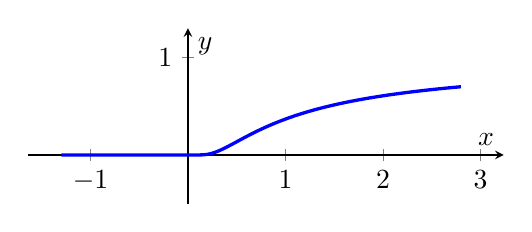
\begin{tikzpicture}[
  declare function={
    func(\x)= (\x <= 0) * (0)   +
              (\x > 0) * (e^(- 1 / \x))
   ;
  }
]
\begin{axis}[
  axis x line=middle, axis y line=middle,
  ymin=-0.5, ymax=1.3, ytick={-1,0,1}, ylabel=$y$,
  xmin=-1.6, xmax=3.2, xtick={-1,...,3}, xlabel=$x$,
  domain=-1.3:2.8,samples=200, % added
  axis equal, height=1.5in, width=3in
]

\addplot [blue,line width=1.2pt] {func(x)};
\end{axis}
\end{tikzpicture} 
    \caption{the function defined in \eqref{eq:smooth-zero-func}, which is smooth at $0$}
    \label{fig:smooth-zero-func-plt}
\end{figure}

Recall that the function \begin{equation} \label{eq:smooth-zero-func}
    f(x) = \begin{cases}
        \exp(-1/x) & \text{if }x > 0, \\
        0 & \text{if }x \leq 0.
    \end{cases}
\end{equation} is a smooth function from $\R$ to $[0,1)$; see \cref{fig:smooth-zero-func-plt}. Now for any $a < b$, consider \begin{equation}
    g(x) = \frac{f(b - x)}{f(b - x) + f(x - a)}. \label{eq:transition-func}
\end{equation} % add plot for g and h
It is clear that $g$ is smooth (the denominator is nowhere zero) and increasing on $\R$, with $g(x) = 1$ when $x \leq a$ and $g(x) = 0$ when $x \geq b$. Such a function $g$ is usually called a \df{transition function}, for the obvious reason.
\begin{figure}
    \centering
        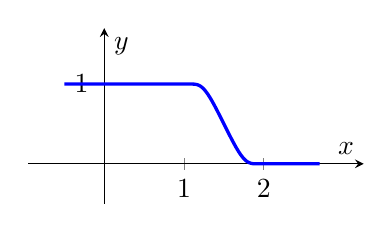
\begin{tikzpicture}[
  declare function={
    f(\x)= (\x <= 0) * (0)   +
              (\x > 0) * (e^(- 1 / \x))
   ;
   g(\x) = f(2 - \x)/(f(2 - \x) + f(\x - 1));
  }
]
\begin{axis}[
  axis x line=middle, axis y line=middle,
  ymin=-0.5, ymax=1.7, ytick={0,1}, ylabel=$y$,
  xmin=-0.7, xmax=3, xtick={0,...,2}, xlabel=$x$,
  domain=-0.5:2.7,samples=200, % added
  axis equal, height=1.5in, width=2.3in
]

\addplot [blue,line width=1.2pt] {g(x)};
\end{axis}
\end{tikzpicture} 
    \caption{the transition function defined in \eqref{eq:transition-func}, when $a = 1$ and $b = 2$}
    \label{fig:transition-func-plt}
\end{figure}

Let $0\leq a < b$, then the function $h\colon x \mapsto g(\nm{x}_2)$ is a smooth function that is $1$ on $\clos{B}(0;a)$ and $0$ outside ${B}(0;b)$. Alternatively if we define $h$ using the max norm instead of the Euclidean norm, then the closed balls should be replaced by closed cubes.
\begin{figure}
    \centering
        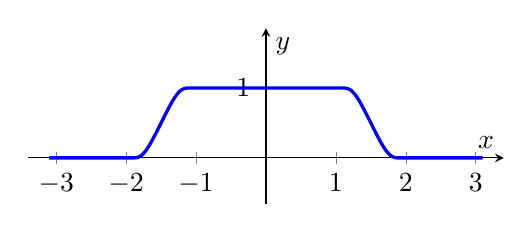
\begin{tikzpicture}[
  declare function={
    f(\x)= (\x <= 0) * (0)   +
              (\x > 0) * (e^(- 1 / \x))
   ;
   g(\x) = f(2 - \x)/(f(2 - \x) + f(\x - 1));
   h(\x) = g(abs(\x));
  }
]
\begin{axis}[
  axis x line=middle, axis y line=middle,
  ymin=-0.5, ymax=1.7, ytick={0,1}, ylabel=$y$,
  xmin=-3.4, xmax=3.4, xtick={-3,...,3}, xlabel=$x$,
  domain=-3.1:3.1,samples=400, % added
  axis equal, height=1.5in, width=3in
]

\addplot [blue,line width=1.2pt] {h(x)};
\end{axis}
\end{tikzpicture} 
    \caption{the bump function defined by $h$ in dimension $1$}
    \label{fig:smooth-bump-func-plt}
\end{figure}

The transition functions and the bump functions are very important approximants to other functions, e.g., indicator functions. The following smooth bump function also appears frequently in the literature as an approximant, because of its straightforward formula. Compose the function $x \mapsto 1 - \nm{x}^2$ with the function $f$ defined in \eqref{eq:smooth-zero-func}, we get a new smooth function \[
    \hat f(x) = \begin{cases}
        \exp\bigl(\frac{1}{\nm{x}^2 - 1}\bigr) & \text{if }\nm{x} < 1, \\
        0 & \text{if }\nm{x} \geq 1,
    \end{cases}
\] which has a closed ball/cube as its support, depending on the norm used.

We remark that $C_c^\infty(\C)$ functions must be the zero function due to Liouville's theorem, in stark contrast to the real case.

\begin{prop}[{\cite[Proposition~8.6]{folland1999}}] \leavevmode
\begin{enumerate} 
    \item $f * g = g * f$.
    \item $f * (g * h) = (f * g) * h$.
    \item $\tau_z (f * g) = (\tau_z f) * g = f * (\tau_z g)$.
    \item $\supp f * g \subseteq \clos{\supp f + \supp g}$.
\end{enumerate}
\end{prop}

In PDE theory, we are interested in functions defined on an open subset $U$ of $\R^n$; however, it can be hard to prove results directly about functions defined such $U$'s. We establish tools for functions defined on the entire $\R^n$, and then use extension and restriction arguments to specialize down to functions defined on $U$.

\cite[Proposition~4.20]{Brezis_2011} proves the second part directly

\begin{prop}[{\cite[Proposition~8.10, Exercise~8.7]{folland1999}}]
    For $f \in L^1(\R^n)$ and $g\in C^k_b(\R^n)$ (i.e., $\partial^\alpha g$ is bounded for all $\abs{\alpha} \leq k$), we have $f * g \in C^k(\R^n)$ with \[
        \partial^\alpha (f * g) = f * (\partial^\alpha g) \text{ for all } \abs{\alpha} \leq k.
    \] 

    If $f \in \locint(\R^n)$ and $g \in C_c^\infty(\R^n)$, then the same claim still holds.
\end{prop}
\begin{proof}
    The first part of theorem is really just differentiation under the integral sign of parameterized functions, \cref{cor:diff-int}.

    The second part of the theorem 
\end{proof}



\cite[Lemma~19.22]{Jost_2005}
For $f \in L^1(U)$, for any open set $V \subseteq \clos{V} \subseteq U$ and $\epsilon < \dist(V,\partial U)$, we have $f^\epsilon \in C^\infty (V)$.

Extend $f$ to $\R^n$ by defining it to be $0$ outside $U$. Then we may see $f \in L^1(\R^n)$

We now introduce the notion of a mollifier. It can smooth out functions, and allows us to approximate a given function by its smoothed-out versions.

Dividing $\hat f$ by a constant, we obtain a function $\eta \in C_c^\infty$ with $\int \eta = 1$. Define $\eta_\epsilon(x) = \frac{1}{\epsilon^n} \eta(x/\epsilon )$ for all $\epsilon > 0$. Then $\eta_\epsilon$ continues to be smooth, $\int \eta_\epsilon = 1$, and now with support contained in $\clos{B}(0;\epsilon)$. The collection $\{\eta_\epsilon\}_{\epsilon \geq 0}$ is an \df{approximation to the identity}. (converges to the Dirac delta function in the Schwartz sense) The function $\eta$ is called the \df{standard mollifier}.

Given $f\in \locint(U)$, define $f^\epsilon = f * \eta_\epsilon$ in the open set $U_\epsilon = \{x \in \R^d : \dist(x,\partial U) > \epsilon\}$.

$f^\epsilon \in C^\infty(U_\epsilon)$
$f^\epsilon \to f$ a.s.\ as $\epsilon \to 0$
uniformly on compact subsets of $U$

For any open set $U \subseteq \R^n$, $C_c^\infty(U)$ is dense in $C_c(U)$, and hence dense in $C_0(U)$.

extend $C_c^\infty(U)$ to $C_c^\infty(\R^n)$,



This tells us that the \nameref{thm:Riesz2} holds for $C_c^\infty$ test functions when the space $X$ considered is $\R^n$.

given $f \in C_c$, consider $f^\epsilon$

$C_c^\infty$ dense in $L^p$ for $1  \leq p < \infty$

% \cite[Proposition~8.17]{folland1999}

\emph{Fundamental theorem of calculus of variation}

\begin{thm}
    For $f \in \locint(U)$, if \[\int f g = 0\] for all $g \in C_c^\infty(U)$, then $f \equiv 0$ on $U$.
\end{thm}

\begin{defn}
    
\end{defn}


\subsection{Spaces of test functions}

Let $X$ be any (Hausdorff) topological space. We define $C_c(X)$ to be the space of continuous functions on $X$ with compact support. We also define $C_0(X)$ to be the space of continuous functions on $X$ such that $\{x:\abs{f(x)} \geq \epsilon\}$ is compact\footnote{The compactness stated here should be viewed as a generalization of boundedness when the space concerned does not have any metric.} for all $\epsilon > 0$.

Since $C_c$ and $C_0$ are both subsets of $C_b$, it is natural to endow the uniform norm $\nm{\blank}_u$ on the two new spaces, and we will always do this henceforth. It turns out quite naturally that $C_0(X)$, as a closed normed subspace of $C_b(X)$, is complete.

In analysis one is often interested in test function classes $C_0$ or $C_c$. Below is one reason why the choice of $C_b$ is desirable to probabilists. Suppose the sequence $\{\mu_n\} \subseteq \mathcal{P}(S)$ converges weakly to $\mu\in \M(S)$. If we take $f = 1$ on the entire $S$ in \eqref{eq:wkconv-def}, then we have $\mu(S) = \lim_n \mu_n(S) = 1$, thus proving that the weak limit $\mu$ is a Borel probability measure as well. Hence no ``mass'' is lost in this convergence, in contrast to ...

We use $\M(S)$ for the space of finite signed/complex Borel measures on $S$, $\M_+(S)$ for the space of finite positive Borel measures on $S$
\begin{defn}
    A sequence $\{\mu_n\}$ is said to 
    \begin{enumerate}
        \item \df[convergence!weak]{converge weakly} to $\mu$ if for all $f\in C_b(S)$, we have \begin{equation}
        \int_S f\,d\mu_n \to \int_S f\,d\mu, \label{eq:wkconv-def}
    \end{equation}
    which we denote by $\mu_n \wkconv \mu$;
    \item \df[convergence!vague]{converge vaguely} to $\mu$ if for all $f\in C_c(S)$, we have \begin{equation}
        \int_S f\,d\mu_n \to \int_S f\,d\mu. \label{eq:vgconv-def}
    \end{equation}
    \end{enumerate}
\end{defn}

It is common to see the notation $\mu f$ in place of $\int_S f\,d\mu$, because we may see $\mu$ as a linear operator acting on the space $C_b(S)$ with the topology of uniform convergence. The bounded continuous functions in the definition are called \df{test functions}, because this mode of convergence is tested with respect to $C_b(S)$.

Weak convergence is a subject of greater importance to probability compared to general measure theory and analysis. This has led to our choice (and many authors' choice) to present weak convergence solely in the context of probability. % A brief overview of the general theory of weak convergence has been included in \cref{sec:weak-conv-general-meas}, based on \cite{Bogachev_2018}.

If $X$ is second countable topological space, then $C_c(X)$ is separable. It follows that its uniform closure $C_0(X)$ is also separable.

Let $X$ be locally compact. If $\sup_n \nm{\mu_n} < \infty$, then it is equivalent to say $\int_S f\,d\mu_n \to \int_S f\,d\mu$ either over all $f \in C_c(X)$ or over all $f \in C_0(X)$, as a consequence of \cref{prop:strong-op-top-dense-subset}. In particular this applies to the space of subprobability measures.


loss of mass at infinity

\begin{defn}
    Let $X$ be an LCH space. A positive \df{Radon measure} $\mu$ on $X$ is a Borel measure that is locally finite, outer regular on all Borel sets, and compact inner regular on all open sets.
\end{defn}

Also may known as \emph{Borel regular measure} or \emph{Riesz measure}

\begin{prop}
    Every Radon measure is compact inner regular on $\sigma$-finite Borel sets. In particular, every $\sigma$-finite Radon measure is compact inner regular on all Borel sets.
\end{prop}

Since we are in a Hausdorff space, a compact inner regular measure is also closed inner regular, and because the measure is finite, it is also outer regular. \textcite{Bogachev_2007,Bogachev_2018} defines a signed measure to be inner regular

Indeed, for finite measures, Radon measures are the same as compact inner regular measures.

\begin{prop}
    Every locally finite Borel measure on an lcscH space is compact inner regular on all Borel sets, and is hence a Radon measure.
\end{prop}

On an lcscH spcae, finite/signed/complex Borel measures are always Radon.

Hence we may identify $\M(X)$ with the space of linear functionals on $C_c(X)$. This allows us to define the weak-star topology on $\M(X)$ by defining the convergence $\mu_n \to \mu$ in $\M(X)$ if \[
    \int f\,d\mu_n \to \int f\,d\mu \quad \text{for all }f \in C_c(X).
\] 

In notation we can write $\sigma\bigl(\M(X), C_c(X) \bigr)$

In fact, this allows us to define a weak-star topology on $\M(X)$. It is clear that $\mu_n \to \mu$ in the weak-star sense if and only if 

% \begin{namedthm}[Riesz–Markov–Kakutani theorem for compact metric spaces]
%     Let $(X,d)$ be a locally compact metric space\footnote{Every compact metric space is separable.}, then the dual space $C(X)^*$ is isometrically isomorphic to $\M(X)$, i.e., for all linear functionals $L \in C(X)^*$, there is a unique $\mu \in \M(X)$ such that \[
%         L(f) = \int_X f\,d\mu\quad \text{for all }f\in C(X);
%     \] meanwhile $\nm{L} = \nm{\mu}$.
% \end{namedthm}

\begin{namedthm}[Riesz--Markov--Kakutani theorem for positive measures] \label{thm:Riesz1}
    
\end{namedthm}

\begin{namedthm}[Riesz--Markov--Kakutani theorem for finite measures] \label{thm:Riesz2}
    Let $X$ be a locally compact metric space, then the dual space $C_c(X)^*$ is isometrically isomorphic to $\M_\mathrm{R}(X)$, i.e., for all linear functionals $L \in C_c(X)^*$, there is a unique signed/complex inner regular Borel measure $\mu$ such that \[
        L(f) = \int_X f\,d\mu\quad \text{for all }f\in C_c(X);
    \] meanwhile $\nm{L} = \nm{\mu}$.

    In particular, if $X$ is separable, then in the above statement $\M_\mathrm{R}(X) = \M(X)$; if furthermore $X$ is compact,\footnote{Compact metric spaces are obviously Lindelöf, and hence separable; see \cref{prop:2nd-count-separable-lindlof}.} then $C_c(X) = C(X)$.

    Every instance of $C_c(X)$ above can be replaced by its uniform closure $C_0(X)$.
\end{namedthm}
% https://math.stackexchange.com/questions/184766/when-is-c-0x-separable

% finite Radon measure (Bogachev 7.1)

% In particular, if $X$ is further assumed to be second countable, then the space of Radon measures $\M_r(X)$ above is just the space of Borel measures $\M(X)$.

vague limit of Radon measures is Radon, and when $\mu_n$ are all positive measures, then the vague limit $\mu$ is positive. To see this, take $f$ to be any nonnegative $C_b$ function. Then $\int f\,d\mu_{n} \to \int f\,d\mu \geq 0$, enforcing $\mu(X) \geq 0$.

\begin{cor}
    $\M_\mathrm{R}(X)$ is a closed subspace of $\M(X)$ and hence a Banach space.
\end{cor}

\begin{prop}
    In a locally compact metric space $X$ with $\mu_n \in \M_r^{+}(X)$ such that $\mu_n \to \mu$, one has $\mu(X) \leq \liminf_n \mu_n (X)$. If $\mu_n$ is allowed to be signed, then $\abs{\mu}(X) \leq \liminf_n \abs{\mu_n} (X)$.
\end{prop}

If one is familiar with Banach space theory, this is an immediate consequence of the \flcnameref{thm:unif-bdd-principle}.

\section{Fourier series}

\section{Fourier transform of functions and measures}

\section{Laplace transform}

% \section{Sobolev spaces}